% This is samplepaper.tex, a sample chapter demonstrating the
% LLNCS macro package for Springer Computer Science proceedings;
% Version 2.20 of 2017/10/04
%
\documentclass[runningheads]{llncs}
%
\usepackage{apacite}
\usepackage{graphicx}
\usepackage{amsmath}
\usepackage{amsfonts}
\usepackage{float}

% Used for displaying a sample figure. If possible, figure files should
% be included in EPS format.
%
% If you use the hyperref package, please uncomment the following line
% to display URLs in blue roman font according to Springer's eBook style:
% \renewcommand\UrlFont{\color{blue}\rmfamily}

\begin{document}
%
\title{White Wine Quality}
\subtitle{Predicci{\'o}n utilizando redes neuronales feedforward\footnote{https://github.com/eadomenech/WineQuality }}
%
%\titlerunning{Abbreviated paper title}
% If the paper title is too long for the running head, you can set
% an abbreviated paper title here
%
\author{Maite S{\'a}nchez-Fornaris\inst{1}\orcidID{0000-0003-3709-9668} \and
Ernesto Avila-Domenech\inst{2}\orcidID{0000-0002-4797-289X}}
%
\authorrunning{M. S{\'a}nchez-Fornaris and E. Avila-Domenech}
% First names are abbreviated in the running head.
% If there are more than two authors, 'et al.' is used.
%
\institute{Universidad de Camag{\"u}ey ``Ignacio Agramonte Loynaz'', Camag{\"u}ey, Cuba.  \email{\{maite.sanchez\}@reduc.edu.cu}\\ \and
Universidad de Granma, Carretera Central v{\'i}a Holgu{\'i}n Km $\frac{1}{2}$, Granma, Cuba \email{\{eadomenech\}@gmail.com}}
%
\maketitle              % typeset the header of the contribution
%
\begin{abstract}
Wine quality certification is of vital importance for wine companies as it guarantees a higher sales and price of the product, as well as preventing it from being adulterated in the distribution chain. Machine learning techniques offer numerous advantages to improve wine quality certification, among the most used models are linear regressions, neighborhood support machines (SVM) and artificial neural networks, which so far have obtained the best results. In this paper, two neural network architectures are proposed for predicting the quality of white wine using the dataset published by the Portuguese company Vinho Verde, which offers 4898 wine samples with 11 characteristics for predicting quality, according to a scale of 7 categories. The expected results were quite good according to the training error calculated through cross entropy, with a high precision.

\keywords{Artificial Neural Network \and White Wine Quality.}
\end{abstract}
%
%
%
\section{Introducci{\'o}n}
El mercado actual tanto a nivel local como global est{\'a} saturado de productos de diferentes marcas en cantidad abrumadoras. Para cualquier empresa constituye todo un reto posicionar sus productos a la vanguardia de estos mercados, siendo requisito indispensable garantizar la calidad del bien que se est{\'a} comercializando. Entonces, ?`c{\'o}mo lo hacen? Pues a nivel internacional existen ciertos organismos que certifican y avalan la calidad de los productos, procesos o servicios. Este es un proceso engorroso por la cantidad de compa\~{n}{\'i}as que los solicitan y la poca disponibilidad de personal para realizar la tarea, adem{\'a}s de que los datos son subjetivos hasta cierto punto para algunos productos \cite{ye2020new}.

La industria del vino, representada fuertemente por Francia, Espa\~{n}a y Portugal, se destaca en este contexto por la complejidad de su proceso para certificar la calidad del vino y la necesidad que tienen de {\'e}l. La certificaci{\'o}n de la calidad del vino aumenta exponencialmente el valor del producto, protegiendo y garantizando su calidad, impide la adulteraci{\'o}n del vino y permite un mejor control en la l{\'i}nea de producción \cite{er2016classification}⁠. Las compa\~{n}{\'i}as vin{\'i}colas se aseguran de certificar la calidad del vino que producen seg{\'u}n dos tipos de pruebas: primero una f{\'i}sico-qu{\'i}mica y la segunda sensorial \cite{radosavljevicdata}⁠, la primera se realiza mediante ex{\'a}menes de laboratorio, sin embargo la segunda requiere de la participaci{\'o}n de personal experto calificado y sus resultados son subjetivos y a{\'u}n no se han comprendido del todo \cite{ye2020new}⁠.

En este contexto, muchas de estas empresas se han apoyado en las t{\'e}cnicas de machine learning para mejorar los resultados de la certificaci{\'o}n de calidad del vino y acelerar el proceso en funci{\'o}n de obtener un mejor producto en el menor tiempo posible con la calidad necesaria \cite{ramazanrole}⁠. Este es el caso de \cite{vlassides2001using}⁠ que utilizaron una red neronal para clasificar vino en California, dado el nivel de maduraci{\'o}n de la uva y los an{\'a}lisis qu{\'i}micos con una muestra de 36 ejemplos y obtuvieron un 6\% de error. En \cite{yu2008prediction}⁠ clasificaron 147 botellas de vino de arroz en 3 categor{\'i}as utilizando mediciones espectrales. Las t{\'e}cnicas m{\'a}s utilizadas han sido las de regresi{\'o}n lineal, las m{\'a}quinas de soporte vectorial (SVM) y {\'u}ltimamente las redes neuronales. La regresi{\'o}n lineal tiene la ventaja de ser sencilla de implementar y de interpretar los resultados, sin embargo no es la m{\'a}s exacta. Las m{\'a}quinas de soporte vectorial dan buenos resultados, pero son f{\'a}cilmente superadas por las redes neuronales artificiales que hasta el momento son las que mejores resultados han obtenido en este tipo de problemas de clasificaci{\'o}n \cite{er2016classification}⁠. 

\section{Descripci{\'o}n del problema}
El problema actual fue planteado por primera vez por \cite{cortez2009modeling} ⁠y est{\'a} dado por la necesidad de utilizar un sistema de apoyo a la toma de decisiones para mejorar el proceso de producci{\'o}n del vino por la compa\~{n}{\'i}a portuguesa Vinho Verde. Portugal es uno de los pa{\'i}ses m{\'a}s importantes en la industria del vino, controlando el 3.17\% en ese mercado. La compa\~{n}{\'i}a Vinho Verde en el momento de la recogida de los datos experimentaba un crecimiento en sus ventas de un 36\%, vi{\'e}ndose en la posici{\'o}n de requerir tecnolog{\'i}a que mejore el proceso de producci{\'o}n, aumente la calidad de sus productos y reduzca los costos de producción.

La empresa contaba con datos hist{\'o}ricos de la calificaci{\'o}n de sus vinos blancos y rojos seg{\'u}n los an{\'a}lisis f{\'i}sico-qu{\'i}micos efectuados en el laboratorio, así como la valoración de los expertos en el análisis sensorial, que esta {\'u}ltima no se public{\'o} por razones de respeto a la privacidad. En esta investigaci{\'o}n se utiliza el conjunto de 4898 muestras del vino blanco Vinho Verde para determinar su calidad, que se describe mediante 7 categor{\'i}as.

Las variables de entrada identificadas en el problema son:
\begin{enumerate}
	\item fixed acidity
	\item volatile acidity
	\item citric acid
	\item residual sugar
	\item chlorides
	\item free sulfur dioxide
	\item total sulfur dioxide
	\item density
	\item pH
	\item sulphates
	\item alcohol3
\end{enumerate}

En el dataset se evidencia poca correlaci{\'o}n entre las variables de entrada, excepto entre los atributos alcohol, sulphates y pH, aunque tampoco es muy alta. La cantidad de alcohol muestra una fuerte relaci{\'o}n positiva con la calidad del vino. En cambio citric acid, free sulfur dioxide, sulphates tiene muy poca o ninguna relaci{\'o}n con la calidad.

\begin{figure}
	\begin{center}
		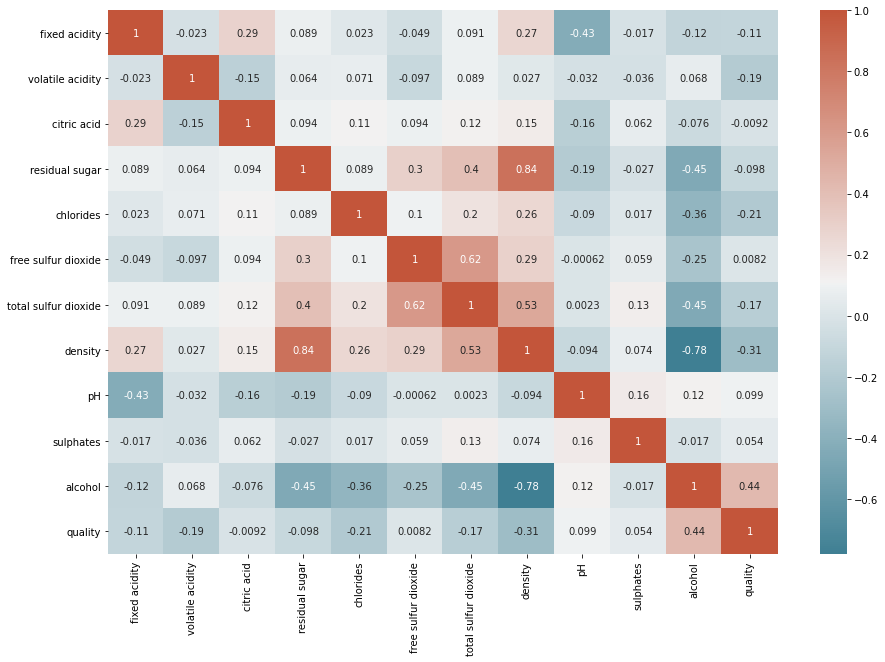
\includegraphics[width=1\textwidth]{images/matrix.png}
		\caption{Correlaci{\'o}n entre los atributos del dataset del vino blanco.} \label{matrix}
	\end{center}
\end{figure}

La variable de salida identificada en el problema es:

quality: Describe la calidad del vino con valores comprendidos en el conjunto \{3, 4, 5, 6, 7, 8, 9\}.

El dataset no contiene valores nulos. Las 11 variables de entrada son de dominio cont{\'i}nuo y la variable de salida es de tipo ordinal, con una relaci{\'o}n de orden ascendente y el valor m{\'a}s representativo en la categor{\'i}a 6, como se muestra en la siguiente figura:

\begin{figure}
	\begin{center}
		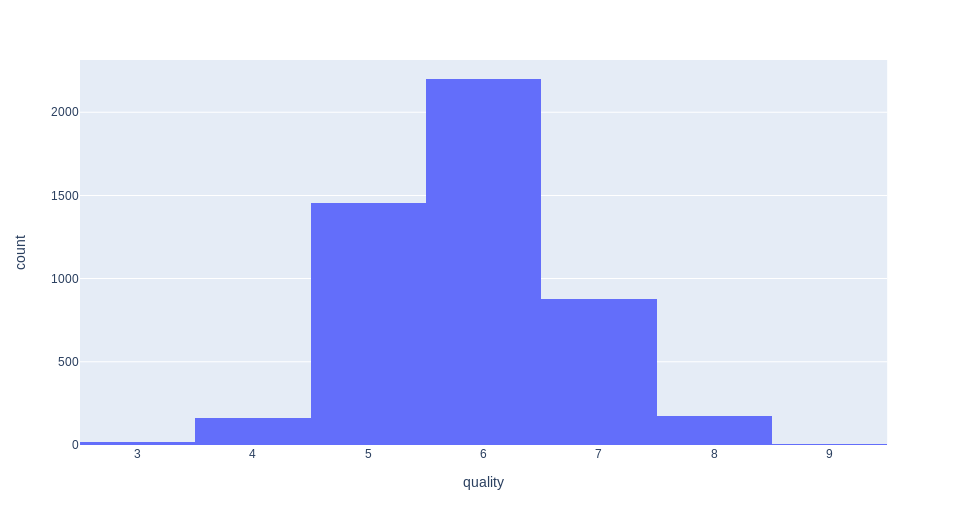
\includegraphics[width=1\textwidth]{images/newplot.png}
		\caption{Distribuci{\'o}n de la clasificaci{\'o}n de la calidad del vino blanco en el dataset.} \label{matrix}
	\end{center}
\end{figure}

\section{Descripci{\'o}n de la soluci{\'o}n.}

\subsection{Preprocesamiento de los datos}
Se aplic{\'o} una normalizaci{\'o}n a los datos debidos a la amplitud y diversidad de rangos de valores en los datos de entrada. Estos se hicieron mediante el m{\'e}todo fit\_transform(x) de la biblioteca sklearn, este m{\'e}todo combina fit() y transform() que se utilizan para centrar o caracterizar la escala de un dato dado. B{\'a}sicamente, ayuda a normalizar los datos dentro de un rango particular. Para ello, utilizan el m{\'e}todo Z-score \cite{raschka2015python}⁠.

\begin{figure}
	\begin{center}
		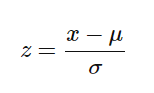
\includegraphics[width=0.2\textwidth]{images/for1.png}
	\end{center}
\end{figure}

Y b{\'a}sicamente encadenan ambos m{\'e}todos de la siguiente forma:

\begin{enumerate}
	\item Fit(): el m{\'e}todo calcula los par{\'a}metros μ y σ y los guarda como objetos internos.
	\item Transform(): el m{\'e}todo que utiliza los par{\'a}metros μ y σ calculados previamente, luego aplica la transformaci{\'o}n a un conjunto de datos en particular.
	\item Fit\_transform(): une el m{\'e}todo fit() y transform() para la transformaci{\'o}n del conjunto de datos.
\end{enumerate}

\begin{figure}
	\begin{center}
		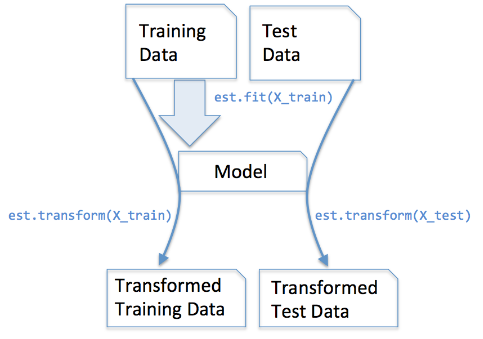
\includegraphics[width=0.6\textwidth]{images/funcionamiento.png}
		\caption{Funcionamiento del m{\'a}todo fit\_transform(x) de sklearn.} \label{matrix}
	\end{center}
\end{figure}

\subsection{Arquitectura de la Red Neuronal Artificial}

Se proponen dos arquitecturas de redes neuronales, la primera de ellas comprende 4 capas completamente conectadas:

\begin{description}
	\item[Capa 1:] 100 neuronas
	\item[Capa 2:] 320 neuronas
	\item[Capa 3:] 100 neuronas
	\item[Capa 4:] 7 neuronas
\end{description}

A cada capa se aplic{\'o} una funci{\'o}n de activación ReLU, para la funci{\'o}n de costo se utiliz{\'o} Cross Entropy Loss y como optimizador se empleó descenso del gradiente estocástico (SGD).

Como funci{\'o}n de activaci{\'o}n se escogi{\'o} ReLU (Rectified Linear Unit) que transforma los valores introducidos anulando los valores negativos y dejando los positivos tal y como entran. Esta funci{\'o}n a\~{n}ade no linealidad a la neurona para mejorar la salida de la red neuronal \cite{jurado2020modelos}⁠.

\begin{figure}
	\begin{center}
		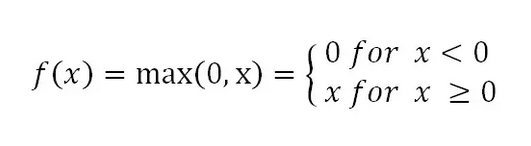
\includegraphics[width=0.6\textwidth]{images/relu.png}
		\caption{Funci{\'o}n ReLU.} \label{relu}
	\end{center}
\end{figure}

Caracter{\'i}sticas de la funci{\'o}n ReLU:
\begin{itemize}
	\item Activaci{\'o}n Sparse – solo se activa si son positivos.
	\item No est{\'a} acotada.
	\item Se pueden morir demasiadas neuronas.
	\item Se comporta bien con im{\'a}genes.
	\item Buen desempea\~{n}o en redes convolucionales.
\end{itemize}

La funci{\'o}n de p{\'e}rdida cross entropy permite comparar el valor estimado por la red con el valor real de nuestro conjunto de entrenamiento cuando se ha calculado la salida \cite{gonzalez2020improved}⁠:

\begin{figure}
	\begin{center}
		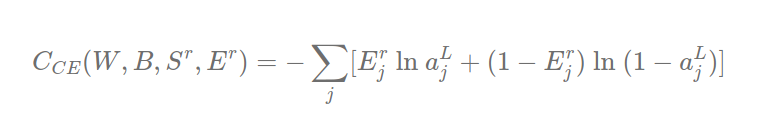
\includegraphics[width=1\textwidth]{images/cross.png}
		\caption{Funci{\'o}n de costo cross entropy.} \label{cross}
	\end{center}
\end{figure}

La funci{\'o}n cross entropy tiene la propiedad de cancelar uno de los t{\'e}rminos dependiendo del valor de la variable de salida y real. El primero cuando el valor real es 0 y el segundo cuando es 1. Existen otras funciones de p{\'e}rdida que se asocian principalmente a redes neuronales profundas.

Una vez que se conoce el error de la estimaci{\'o}n con respecto de la salida real se procede a calcular el ajuste necesario para los pesos de la red, es decir mejorar los par{\'a}metros $W$ y $b$ de las neuronas de la red para que produzcan mejores estimaciones.

El m{\'e}todo cross entropy tiene una estructura sencilla que aplicarse a cualquier problema. Funciona para problemas simples, como la regresi{\'o}n y tambi{\'e}n para problemas m{\'a}s complejos, como el de clasificaci{\'o}n. Es posible notar que para la regresi{\'o}n no produce mejoras significativas pero esto se debe a que son problemas sencillos que ya est{\'a}n optimizados al m{\'a}ximo con los m{\'e}todos tradicionales. Sin embargo, en clasificaci{\'o}n se obtienen resultados mejores que con las soluciones cl{\'a}sicas. Adem{\'a}s, cuanto m{\'a}s complejo sea el problema (m{\'a}s clases, m{\'a}s variables y diferentes tipos de variables) mayor es la mejora del error con este m{\'e}todo.

Como defectos de este m{\'e}todo, s{\'o}lo cabe detacar uno, que es el tiempo de ejecuci{\'o}n, que en parte se puede reducir algo optimizando la red.

En la segunda arquitectura se usaron 3 capas de neuronas completamente conectadas:

\begin{description}
	\item[Capa 1:] 100 neuronas
	\item[Capa 2:] 50 neuronas
	\item[Capa 3:] 7 neuronas
\end{description}

La primera capa se activ{\'o} con una función ReLU y la segunda con una softmax, como funci{\'o}n de p{\'e}rdida se us{\'o} tambi{\'e}n cross entropy y como optimizador el m{\'e}todo de Adam.

La funci{\'o}n softmax es una generalizaci{\'o}n de la funci{\'o}n log{\'i}stica y convierte variables independientes de rango casi infinito en probabilidades simples entre [0,1].

\begin{figure}
	\begin{center}
		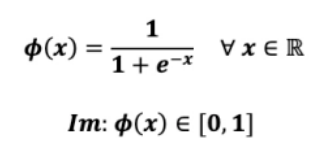
\includegraphics[width=0.5\textwidth]{images/softmax.png}
		\caption{Funci{\'o}n de activaci{\'o}n softmax.} \label{softmax}
	\end{center}
\end{figure}

Soporta sistemas de clasificaci{\'o}n multinomial, por lo que se convierte en el recurso principal utilizado en las capas de salida de un clasificador. Esta funci{\'o}n de activaci{\'o}n devuelve la distribuci{\'o}n de probabilidad de cada una de las clases soportadas en el modelo. La funci{\'o}n softmax calcula la distribuci{\'o}n de probabilidades del evento sobre $n$ eventos diferentes. En t{\'e}rminos generales, esta funci{\'o}n calcular{\'a} las probabilidades de cada clase objetivo sobre todas las clases objetivo posibles. M{\'a}s tarde, las probabilidades calculadas ser{\'a}n {\'u}tiles para determinar la clase objetivo para las entradas dadas.

La principal ventaja de usar softmax es el rango de probabilidades de salida. El rango ser{\'a} de 0 a 1, y la suma de todas las probabilidades ser{\'a} igual a uno. Este tipo de funci{\'o}n de activaci{\'o}n es muy utilizado en el modelo de regresi{\'o}n log{\'i}stica de clasificaci{\'o}n m{\'u}ltiple y en diferentes niveles de capa de cara a la construcci{\'o}n de redes neuronales \cite{ambrogioni2017kernel}⁠.

El optimizador Adam trata de solventar el problema con la fijaci{\'o}n de el ratio de aprendizaje del SGD, para ello adapta el ratio de aprendizaje en funci{\'o}n de c{\'o}mo est{\'e}n distribuidos los par{\'a}metros. Si los par{\'a}metros est{\'a}n muy dispersos (sparse) el ratio de aprendizaje aumentar{\'a}. Adam es una actualizaci{\'o}n del Optimizador RMSProp (Root Mean Square Propagation) que se basa en un ratio de aprendizaje adaptativa.

El algoritmo ADAM seg{\'u}n \cite{kingma2014adam}⁠ calcula la direcci{\'o}n de descenso usando momentum y utiliza una estrategia similar para calcular adaptar el tama\~{n}o de paso. Es decir, utiliza momentum para actualizar el paso, lo que evita cambios bruscos en el mismo. Esto lo hace muy estable para su uso en una estrategia tipo Gradiente Estoc{\'a}stico (SGD) donde las muestras pueden provocar cambios grandes en la magnitud del gradiente, adem{\'a}s calcula un paso global en vez de usar un paso para cada variable. Tambi{\'e}n adecuado en estrategias de entrenamiento tipo estoc{\'a}sticas o por lotes, como en el caso de Redes Neuronales Profundas (Deep Learning). Una mejora importante es la correci{\'o}n del sesgo (bias) en la estimaci{\'o}n de los momentos. Generalmente las razones de aprendizaje (momentum) son cercanas a 1.

\section{Resultados}

En la primera red entrenada con SGD y ratio de aprendizaje de 0.003 con 20 iteraciones se obtuvo un error de entrenamiento de 0.6933326721191406.

Para la segunda variante entrenada con Adam y un ratio de aprendizaje de 0.01 en 100 iteraciones se obtuvo un error de entrenamiento de 0.9620 y una precisi{\'o}n de 56\%.

\begin{figure}[htbp]
	\centering
	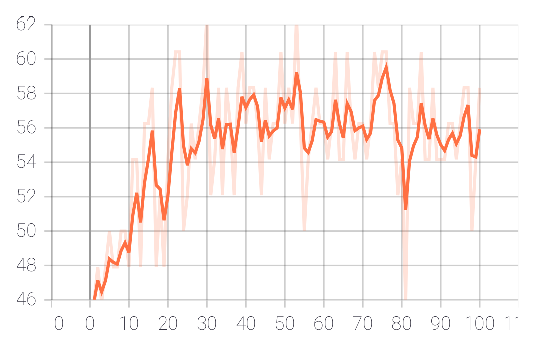
\includegraphics[width=0.5\textwidth]{images/Accuracy.eps}
	\caption{Comportamiento de la precisi{\'o}n durante la predicci{\'o}n en el conjunto de prueba.}
	\label{accuracy}
\end{figure}

\begin{figure}[htbp]
	\centering
	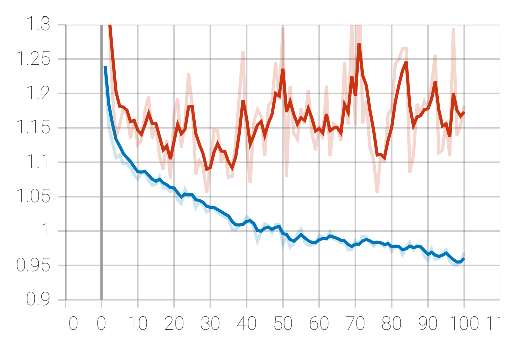
\includegraphics[width=0.5\textwidth]{images/LOSS.eps}
	\caption{Comportamiento de los errores de entrenamiento y validaci{\'o}n.}
	\label{loss}
\end{figure}  

\section{Conclusiones}
Una comprensi{\'o}n cabal de las propiedades f{\'i}sico-qu{\'i}micas del vino blanco es fundamental para tener {\'e}xito en la predicci{\'o}n de su calidad utilizando redes neuronales. Se comprob{\'o} que el grado de alcohol es la caracter{\'i}stica que m{\'a}s se tiene en cuenta para valorar la calidad del vino, en cambio el {\'a}cido c{\'i}trico, el di{\'o}xido de azufre libre y los sulfatos tienen poca o ninguna influencia en la calidad. Como algunas de estas variables f{\'i}sico-qu{\'i}micas pueden controlarse desde el proceso de producci{\'o}n,  la informaci{\'o}n obtenida puede utilizarse para mejorar la calidad del vino desde la f{\'a}brica. Se propusieron dos modelos de redes neuronales y se implementaron utilizando el framework PyTorch, visualiz{\'a}ndose los gr{\'a}ficos con Tensorboard. Con ambos modelos se obtuvieron resultados aceptables.

%
% ---- Bibliography ----
%
% BibTeX users should specify bibliography style 'splncs04'.
% References will then be sorted and formatted in the correct style.
%
\bibliographystyle{apacite}
\bibliography{mybibliography}
%
\end{document}
